% !TEX root = ../master.tex
% =============================================================================
% MASTER PLATFORM CORE: Shared Intent-Based Instructions (Union)
% World-Class Version: HITL Gates, Process Integrity, and .clinerules Wiring
% =============================================================================

\section{Rules of Engagement for AI Agents}
\label{sec:agent-rules}

To ensure safety and architectural integrity, all implementation agents must adhere to the following Prime Directives:

\begin{enumerate}[label=\textsc{rule}-\arabic*:, leftmargin=2cm]
    \item \textbf{Credential Protection.} Never log, print, or commit secrets. Use the \texttt{.secrets.example} pattern for all new integrations.
    \item \textbf{Context Efficiency.} Prioritize surgical edits. Request only the minimum required file ranges to satisfy the task intent.
    \item \textbf{Test-Driven Implementation.} No code is complete without a corresponding fixture in \texttt{tests/fixtures/} and a passing validation run.
    \item \textbf{Self-Correction.} If a schema validation fails, the agent must diagnose the root cause (hallucination vs. schema drift) before re-attempting implementation.
    \item \textbf{Safety Inheritance.} Domain-specific agent rules (\texttt{.clinerules}) may only \emph{tighten} (e.g., lower timeout, stricter precision), never \emph{loosen} regulatory constraints.
\end{enumerate}

\section{Agent Rule-Pack Architecture (.clinerules)}
\label{sec:agent-rule-packs}

The platform mandates a three-tier inheritance hierarchy for agent behavior. Implementation agents must load the relevant rule pack before starting any task.

\subsection{Inheritance Hierarchy}
\begin{enumerate}
    \item \textbf{Repository-level (\texttt{/.clinerules}):} The baseline for all engineering and documentation standards.
    \item \textbf{Intelligence-level (\texttt{/src/intelligence/.clinerules}):} The regulatory envelope (MAS MGF) that wraps all domains.
    \item \textbf{Domain-level (\texttt{/src/<domain>/.clinerules}):} Domain-specific constraints (e.g., Arabic character precision).
\end{enumerate}

\subsection{Safety-Critical Flags}
The following flags in the rule packs are subject to \textsc{rule-5} (Inherit, Never Weaken):
\begin{table}[htbp]
\centering
\footnotesize
\caption{Safety-Critical Agent Flags.}
\label{tab:safety-flags}
\begin{tabularx}{\textwidth}{@{}l X X@{}}
\toprule
\textbf{Flag} & \textbf{Parent Value (Regs)} & \textbf{Tightening Direction} \\
\midrule
\texttt{deny\_by\_default} & \texttt{true} & Invariant (Cannot be set to false). \\
\texttt{require\_identity} & \texttt{true} & Invariant (Cannot be bypassed). \\
\texttt{max\_retries} & \texttt{3} & May only \emph{decrease}. \\
\texttt{timeout\_ms} & \texttt{30000} & May only \emph{decrease}. \\
\bottomrule
\end{tabularx}
\end{table}

\section{Platform Overview --- One Codebase, One Instance}
\label{sec:agent-platform-overview}

\subsection{Integration Stance}
The SAP OSS platform is delivered as a single codebase that runs as a single logical instance. All cross-cutting concerns are hosted by existing services.

\begin{adrbox}{{One Codebase, One Instance}}
To minimize integration latency and eliminate distributed-system failure modes (e.g., partial partitions), we mandate a single logical instance. All cross-domain orchestration happens via the MCP Gateway layer.
\end{adrbox}

\subsection{Platform Integration Map}
\label{sec:platform-map}

\begin{figure}[htbp]
\centering
\begin{tikzpicture}[
    node distance=2.5cm, 
    auto,
    block/.style={rectangle, draw, rounded corners, fill=sapblue!10, text width=6em, text centered, minimum height=3em, font=\scriptsize},
    regs/.style={rectangle, draw, rounded corners, fill=sapgrey!20, text width=7em, text centered, minimum height=4em, thick, dotted, font=\scriptsize}
]
    \node (arabic) [block] {Arabic AP};
    \node (tb) [block, below of=arabic] {Trial Balance};
    \node (simula) [block, right of=arabic, node distance=5.5cm] {Simula Training};
    \node (regs) [regs, below of=simula] {Regulations (Runtime Wrapper)};
    
    \draw [->, thick] (arabic) -- node [align=left, font=\tiny] {Posted\\Invoices} (tb);
    \draw [->, thick, dashed] (simula) -- node [align=left, font=\tiny, near start] {Training\\Examples} (arabic);
    \draw [->, thick, dashed] (simula) -- node [align=left, font=\tiny, near start] {Training\\Examples} (tb);
    \draw [->, thick] (regs) -| node [font=\tiny, near end, xshift=-1cm] {Governance Gate} (arabic);
    \draw [->, thick] (regs) -| node [font=\tiny, near end, xshift=-1cm] {Audit \& Identity} (tb);
\end{tikzpicture}
\caption{Cross-domain interaction and unified data flow map. Detailed governance logic is defined in \cref{reg:ch:mgf}.}
\end{figure}

\section{Transactional Sequence Diagrams}
\label{sec:agent-sequences}

Implementation agents must adhere to the temporal logic defined below. Every cross-domain request MUST be brokered by the Regulations Wrapper.

\subsection{Universal Governance Handshake}
This sequence applies to \textbf{all} platform service calls.

\begin{figure}[htbp]
\centering
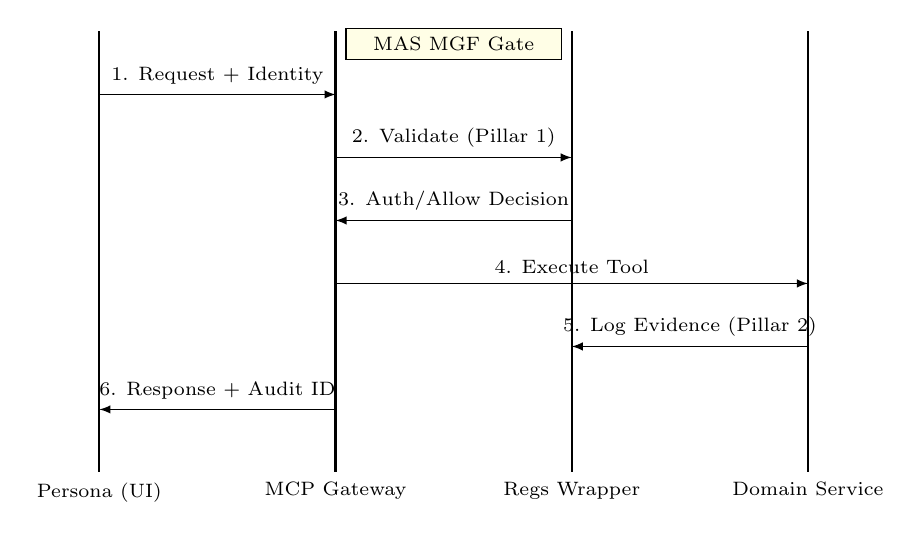
\begin{tikzpicture}[x=1cm, y=-0.8cm, font=\scriptsize]
    % Lifelines
    \draw[thick] (0,0) -- (0,7) node[below] {Persona (UI)};
    \draw[thick] (3,0) -- (3,7) node[below] {MCP Gateway};
    \draw[thick] (6,0) -- (6,7) node[below] {Regs Wrapper};
    \draw[thick] (9,0) -- (9,7) node[below] {Domain Service};

    % Interaction
    \draw[->, >=latex] (0,1) -- node[above] {1. Request + Identity} (3,1);
    \draw[->, >=latex] (3,2) -- node[above] {2. Validate (Pillar 1)} (6,2);
    \draw[<-, >=latex] (3,3) -- node[above] {3. Auth/Allow Decision} (6,3);
    \draw[->, >=latex] (3,4) -- node[above] {4. Execute Tool} (9,4);
    \draw[->, >=latex] (9,5) -- node[above] {5. Log Evidence (Pillar 2)} (6,5);
    \draw[<-, >=latex] (0,6) -- node[above] {6. Response + Audit ID} (3,6);

    \node[draw, fill=yellow!10, text width=2.5cm, align=center] at (4.5,0.2) {MAS MGF Gate};
\end{tikzpicture}
\caption{Standard platform handshake for governed tool execution. Audit schemas are detailed in \cref{reg:ch:identity}.}
\end{figure}

\subsection{Arabic AP Golden Path}
Temporal flow for invoice processing with Arabic context.

\begin{figure}[htbp]
\centering
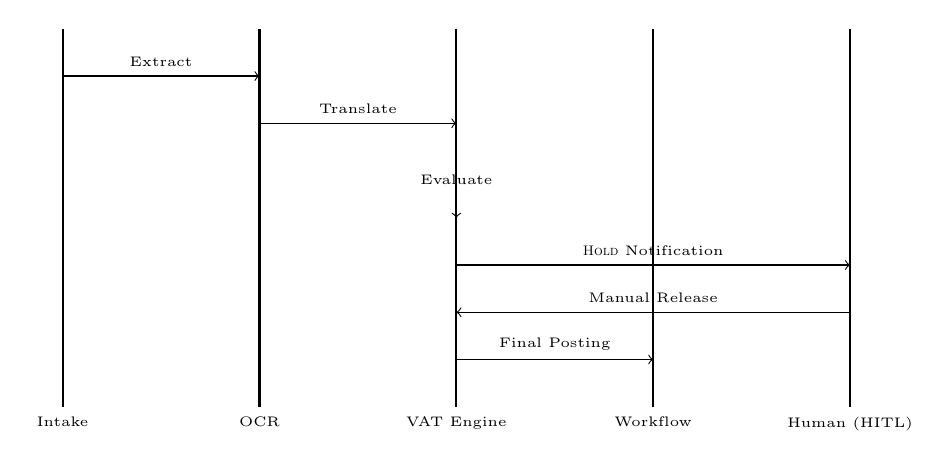
\begin{tikzpicture}[x=1cm, y=-0.6cm, font=\tiny]
    \draw[thick] (0,0) -- (0,8) node[below] {Intake};
    \draw[thick] (2.5,0) -- (2.5,8) node[below] {OCR};
    \draw[thick] (5,0) -- (5,8) node[below] {VAT Engine};
    \draw[thick] (7.5,0) -- (7.5,8) node[below] {Workflow};
    \draw[thick] (10,0) -- (10,8) node[below] {Human (HITL)};

    \draw[->] (0,1) -- node[above] {Extract} (2.5,1);
    \draw[->] (2.5,2) -- node[above] {Translate} (5,2);
    \draw[->] (5,3) -- node[above] {Evaluate} (5,4); % Internal loop
    \draw[->] (5,5) -- node[above] {\textsc{Hold} Notification} (10,5);
    \draw[<-] (5,6) -- node[above] {Manual Release} (10,6);
    \draw[->] (5,7) -- node[above] {Final Posting} (7.5,7);
\end{tikzpicture}
\caption{Arabic AP sequence: Scanned PDF to Release. VAT rules are specified in \cref{ar:ch:vat}.}
\end{figure}

\section{Compute and Resource Alignment}
\label{sec:hardware-profiles}

AI algorithms are calibrated for the reference infrastructure established in the domain chapters:

\begin{table}[htbp]
\centering
\footnotesize
\caption{Infrastructure Reference Profiles.}
\label{tab:hardware-profiles}
\begin{tabularx}{\textwidth}{@{}l X X@{}}
\toprule
\textbf{Workload} & \textbf{Reference Hardware} & \textbf{Performance Target} \\
\midrule
LLM Inference & NVIDIA L40S (48GB) & AWQ 4-bit / p95 < 2s \\
Embeddings & NVIDIA A100 (40/80GB) & FP16 / p99 < 500ms \\
Simula Training & NVIDIA A100 SXM4 cluster & BF16 throughput parity \\
\bottomrule
\end{tabularx}
\end{table}

\section{Human-in-the-Loop (HITL) Critical Gates}
\label{sec:hitl-gates}

The following "Four-Eyes" gates are mandatory. AI agents must implement the "Awaiting Sign-off" state for these actions:
\begin{itemize}
    \item \textbf{VAT Release:} No invoice marked as \textsc{hold} can be released without human review (see \cref{ar:ch:ap}).
    \item \textbf{Anomaly Override:} Statistical outliers ($3\sigma$) cannot be dismissed by AI; only "Confirmed" or "Triaged" by human (see \cref{tb:ch:controls}).
    \item \textbf{Journal Posting:} Agents may \emph{draft} journal entries, but only the Financial Controller persona can \emph{commit} to S/4HANA (see \cref{tb:ch:controls-engine}).
\end{itemize}

\section{Registry Integrity \& Live Status}
\label{sec:registry-integrity}

Before initiating any schema-dependent task, implementation agents must verify the live status of the Unified Schema Registry (see \cref{sim:chap:schema}).
\begin{adrbox}{Registry First}
If \texttt{docs/schema/registry.json} is out of sync with the codebase, the agent must halt and emit a \textsc{schema-mismatch} event.
\end{adrbox}

\section{Master Implementation Manifest (Union)}
Implementation runs in three waves across the entire platform.

\subsection*{Wave 1 --- Foundations}
\begin{itemize}
    \item \textbf{Simula:} Implement HANA schema extraction pipeline (MCP discovery). See \cref{sim:chap:extraction}.
    \item \textbf{Regulations:} Implement MAS MGF Pillar 1 logic (Tool allow-list). See \cref{reg:ch:mgf}.
    \item \textbf{Arabic:} Implement Invoice Intake \& OCR Gateway. See \cref{ar:ch:ai}.
    \item \textbf{Trial Balance:} Implement identity-attribution wiring. See \cref{reg:ch:identity}.
\end{itemize}

\subsection*{Wave 2 --- Core Domain Build-out}
\begin{itemize}
    \item \textbf{Trial Balance:} Implement Controls \& Commentary Engine (3$\sigma$ anomaly logic). See \cref{tb:ch:ai,tb:ch:controls-engine}.
    \item \textbf{Arabic:} Implement multi-country VAT Engine (Saudi, UAE, Bahrain, Oman). See \cref{ar:ch:vat,ar:ch:vat-impl}.
    \item \textbf{Simula:} Implement Taxonomy Generation \& Agentic Data Synthesis. See \cref{sim:chap:taxonomy,sim:chap:generator}.
    \item \textbf{Trial Balance:} Realise 28-state BPMN workflow (\texttt{tb-review-glo}). See \cref{tb:ch:workflow}.
\end{itemize}

\subsection*{Wave 3 --- Hardening}
\begin{itemize}
    \item \textbf{Regulations:} Implement Per-Request Identity Attribution. See \cref{reg:ch:identity}.
    \item \textbf{Trial Balance:} Deliver Human Review Dashboard. See \cref{tb:ch:review-dashboard}.
    \item \textbf{Simula:} Deliver test fixtures and testing at 85\% coverage. See \cref{sim:ch:test-fixtures,sim:ch:testing}.
    \item \textbf{Regulations:} Wire Emergent-Capability monitoring. See \cref{reg:ch:monitoring}.
\end{itemize}

\section{Governance Obligations (MAS MGF)}
The regulations domain wraps all service calls at runtime. Agents must implement the following hooks in every domain:
\begin{itemize}
    \item \textbf{Pillar 1:} Tool allow-list enforcement (deny-by-default).
    \item \textbf{Pillar 2:} Traceability via the identity attribution envelope.
    \item \textbf{Pillar 3:} Metric emission to the monitoring sink.
\end{itemize}
Detailed pillar requirements are defined in \cref{reg:ch:mgf}.
